% !TEX encoding = UTF-8 Unicode
\section{Preventivo}
	\subsection{Dettaglio fasi}
		\subsubsection{Fase A}
			\paragraph{Suddivisione lavoro}
				Nella \insphase{Fase A} ogni componente del gruppo \groupname{} coprirà i seguenti ruoli:
				\begin{table}[H]
					\begin{center}
						\begin{tabular}{| l | c | c | c | c | c | c | c |}
							\hline
							Componente 				& PM	& Am 	& An 	& Pt 		& Pm 	& Ve 	& Ore Totali componente \\ \hline
							
							Bigarella Chiara 			& 0		& 5 		& 30 		& 0		& 0		& 8 		& 43 \\
							Bucco Riccardo 			& 0		& 5 		& 30 		& 0		& 0		& 8 		& 43 \\
							Carlon Chiara	 			& 0		& 6 		& 9 		& 0		& 0		& 17 		& 32 \\
							Dal Bianco Davide 			& 0		& 14 		& 25 		& 0		& 0		& 5 		& 44 \\
							Moretto Alessandro 			& 25 		& 0		& 9 		& 0		& 0		& 8 		& 42 \\
							Pavanello Fabio Matteo	 	& 0		& 5 		& 6 		& 0		& 0		& 23 		& 34 \\
							Rubin Marco				& 7 		& 19 		& 0		& 0		& 0		& 8 		& 34 \\ \hline \hline
							
							Ore Totali Ruolo 			& 32 		& 54 		& 109 	& 0		& 0		& 77 		& 272\\ \hline
						\end{tabular}
					\end{center}
					\caption{Suddivisione ore di lavoro Fase A}
				\end{table}
				Riassumendo con un Bar Chart:
				\begin{figure}[H]\centering
					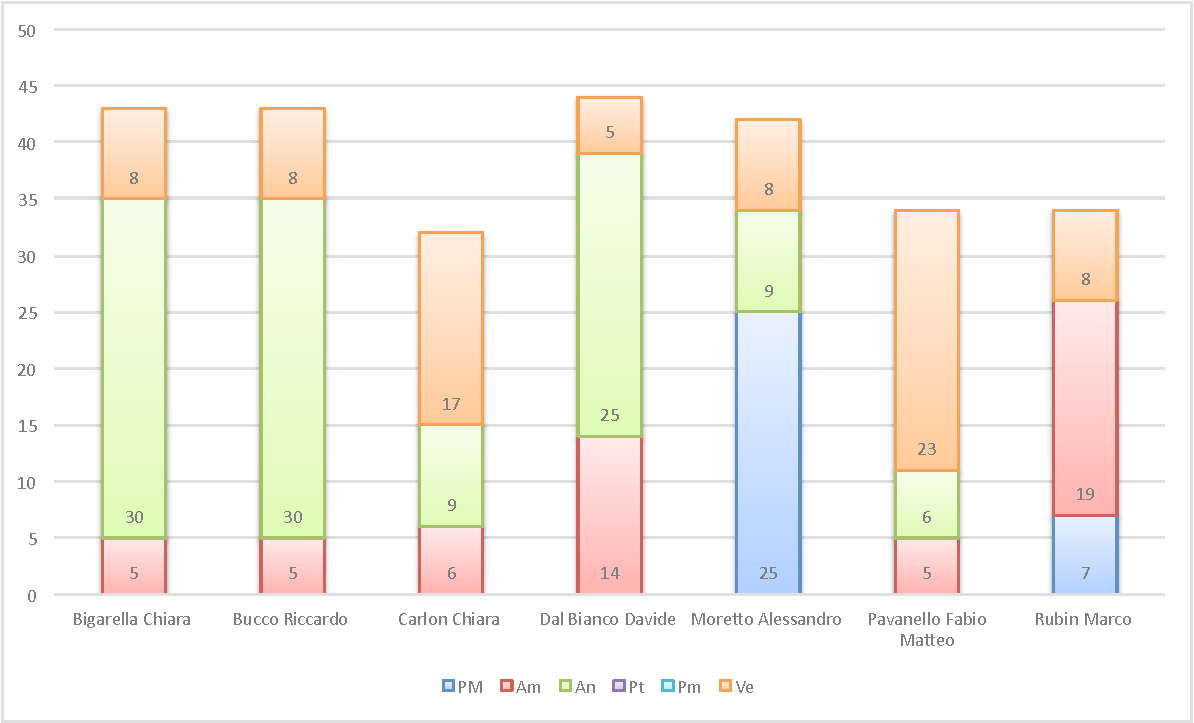
\includegraphics[width=\textwidth]{PianoDiProgetto/Pics/ChartOreFaseA.pdf}
					\caption{Bar Chart ore persona Fase A}
				\end{figure}
			\paragraph{Prospetto economico}
				Nella \insphase{Fase A} il costo di ogni ruolo è il seguente:
				\begin{table}[H]
					\begin{center}
						\begin{tabular}{| l | c | c |}
							\hline
							Ruolo 			& Ore 	& Costi  \\ \hline
							
							Product Manager	& 32 		& \euro{} 960,00 	\\
							Amministratore 		& 54 		& \euro{} 1~080,00 	\\
							Analista	 		& 109 	& \euro{} 2~725,00 	\\
							Progettista 		& 0		& \euro{} 0,00 	\\
							Programmatore		& 0		& \euro{} 0,00	\\
							Verificatore		& 77 		& \euro{} 1~155,00 	\\ \hline \hline
							
							Totale	 		& 272 	& \euro{} 5~920,00 	\\ \hline
						\end{tabular}
					\end{center}
					\caption{Costi per ruolo Fase A}
				\end{table}
				Riassumendo le ore per ruolo con un Cake Chart:
				\begin{figure}[H]\centering
					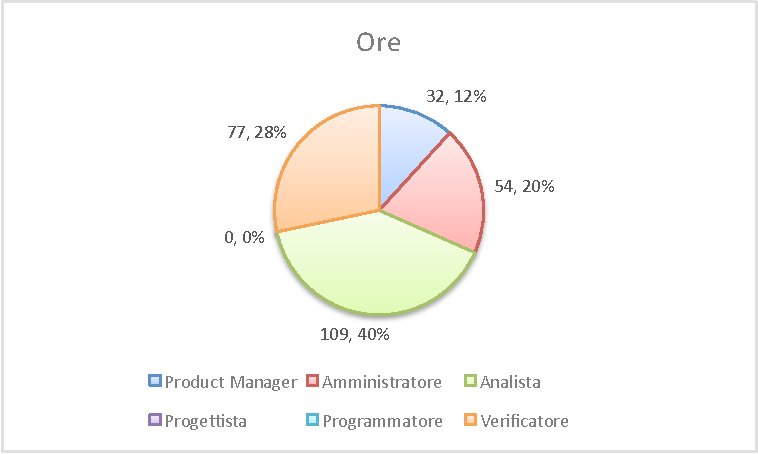
\includegraphics[width=\textwidth]{PianoDiProgetto/Pics/ChartTotOreFaseA.pdf}
					\caption{Cake Chart ore per ruolo Fase A}
				\end{figure}
				Riassumendo i costi per ruolo con un Cake Chart:
				\begin{figure}[H]\centering
					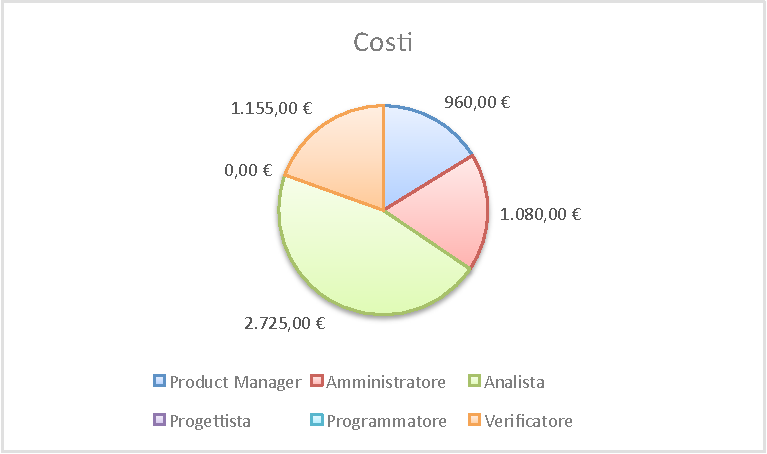
\includegraphics[width=\textwidth]{PianoDiProgetto/Pics/ChartTotCostiFaseA.pdf}
					\caption{Cake Chart costi per ruolo Fase A}
				\end{figure}
		\subsubsection{Fase AD}
			\paragraph{Suddivisione lavoro}
				Nella \insphase{Fase AD} ogni componente del gruppo \groupname{} coprirà i seguenti ruoli:
				\begin{table}[H]
					\begin{center}
						\begin{tabular}{| l | c | c | c | c | c | c | c |}
							\hline
							Componente 				& PM	& Am 	& An 	& Pt 		& Pm 	& Ve 	& Ore Totali componente \\ \hline
							
							Bigarella Chiara 			& 0		& 7 		& 0		& 0		& 0		& 5 		& 12 \\
							Bucco Riccardo 			& 0		& 6 		& 0		& 0		& 0		& 7 		& 13 \\
							Carlon Chiara	 			& 7 		& 0		& 3 		& 0		& 0		& 2 		& 12 \\
							Dal Bianco Davide 			& 0		& 6 		& 0		& 0		& 0		& 5 		& 11 \\
							Moretto Alessandro 			& 0		& 0		& 3 		& 0		& 0		& 8 		& 11 \\
							Pavanello Fabio Matteo	 	& 0		& 0		& 3 		& 0		& 0		& 10 		& 13 \\
							Rubin Marco				& 0		& 0		& 3 		& 0		& 0		& 10 		& 13 \\ \hline \hline
							
							Ore Totali Ruolo 			& 7 		& 19 		& 12 		& 0		& 0		& 47 		& 85\\ \hline
						\end{tabular}
					\end{center}
					\caption{Suddivisione ore di lavoro Fase AD}
				\end{table}
				Riassumendo con un Bar Chart:
				\begin{figure}[H]\centering
					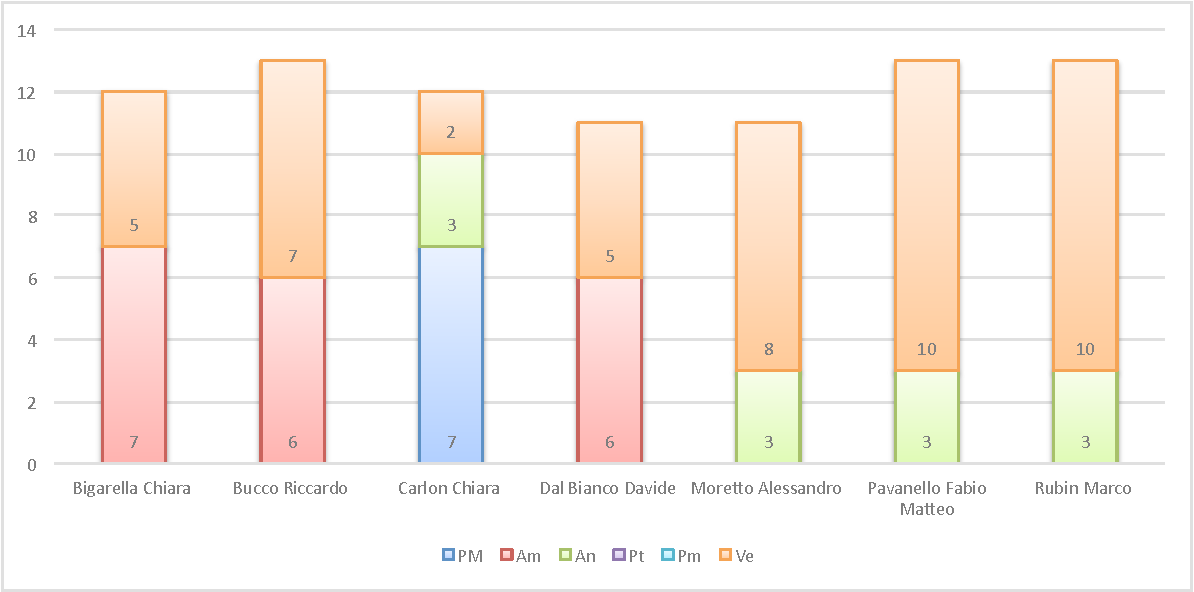
\includegraphics[width=\textwidth]{PianoDiProgetto/Pics/ChartOreFaseAD.pdf}
					\caption{Bar Chart ore persona Fase AD}
				\end{figure}
			\paragraph{Prospetto economico}
				Nella \insphase{Fase AD} il costo di ogni ruolo è il seguente:
				\begin{table}[H]
					\begin{center}
						\begin{tabular}{| l | c | c |}
							\hline
							Ruolo 			& Ore 	& Costi  \\ \hline
							
							Product Manager	& 7 		& \euro{} 210,00 	\\
							Amministratore 		& 19 		& \euro{} 380,00 	\\
							Analista	 		& 12 		& \euro{} 300,00 	\\
							Progettista 		& 0		& \euro{} 0,00 	\\
							Programmatore		& 0		& \euro{} 0,00	\\
							Verificatore		& 47 		& \euro{} 705,00 	\\ \hline \hline
							
							Totale	 		& 85 		& \euro{} 1~595,00 	\\ \hline
						\end{tabular}
					\end{center}
					\caption{Costi per ruolo Fase AD}
				\end{table}
				Riassumendo le ore per ruolo con un Cake Chart:
				\begin{figure}[H]\centering
					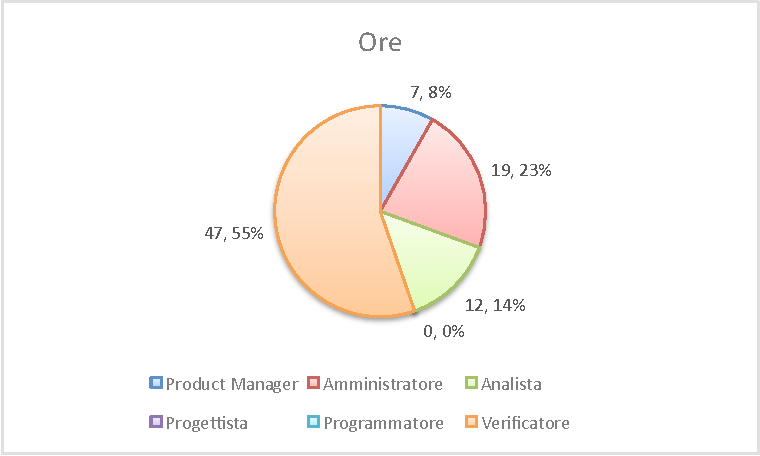
\includegraphics[width=\textwidth]{PianoDiProgetto/Pics/ChartTotOreFaseAD.pdf}
					\caption{Cake Chart ore per ruolo Fase AD}
				\end{figure}
				Riassumendo i costi per ruolo con un Cake Chart:
				\begin{figure}[H]\centering
					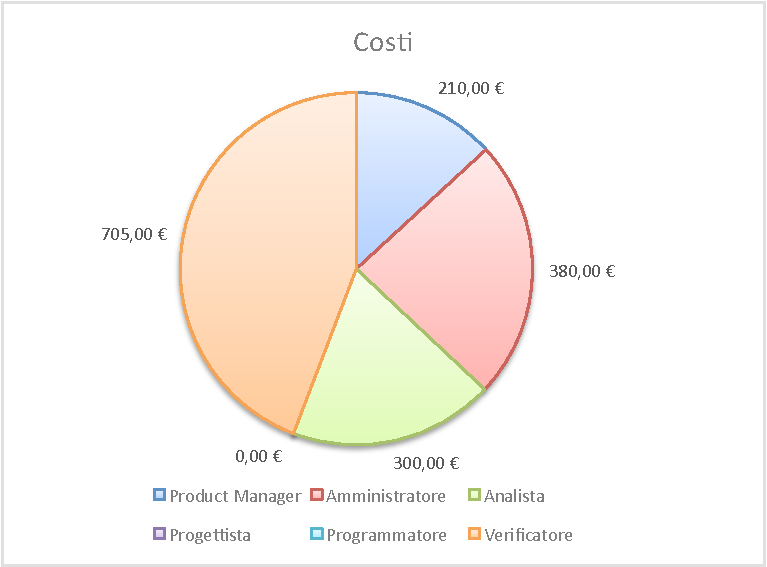
\includegraphics[width=\textwidth]{PianoDiProgetto/Pics/ChartTotCostiFaseAD.pdf}
					\caption{Cake Chart costi per ruolo Fase AD}
				\end{figure}
		\subsubsection{Fase PA}
			\paragraph{Suddivisione lavoro}
				Nella \insphase{Fase PA} ogni componente del gruppo \groupname{} coprirà i seguenti ruoli:
				\begin{table}[H]
					\begin{center}
						\begin{tabular}{| l | c | c | c | c | c | c | c |}
							\hline
							Componente 				& PM	& Am	 & An 	& Pt 		& Pm 	& Ve 	& Ore Totali componente \\ \hline
							
							Bigarella Chiara 			& 0		& 0		& 10 		& 17 		& 0		& 6 		& 33 \\
							Bucco Riccardo 			& 15 		& 0		& 0		& 15 		& 0		& 5 		& 35 \\
							Carlon Chiara	 			& 0		& 7 		& 12 		& 0		& 0		& 9 		& 28 \\
							Dal Bianco Davide 			& 0		& 0		& 0		& 20 		& 0		& 5		& 25 \\
							Moretto Alessandro 			& 0		& 3 		& 10 		& 12 		& 0		& 5 		& 30 \\
							Pavanello Fabio Matteo	 	& 0		& 0		& 25 		& 0		& 0		& 0		& 25 \\
							Rubin Marco				& 9 		& 0		& 12 		& 0		& 0		& 7 		& 28 \\ \hline \hline
							
							Ore Totali Ruolo 			& 24 		& 10 		& 69 		& 64 		& 0		& 37		& 204\\ \hline
						\end{tabular}
					\end{center}
					\caption{Suddivisione ore di lavoro Fase PA}
				\end{table}
				Riassumendo con un Bar Chart:
				\begin{figure}[H]\centering
					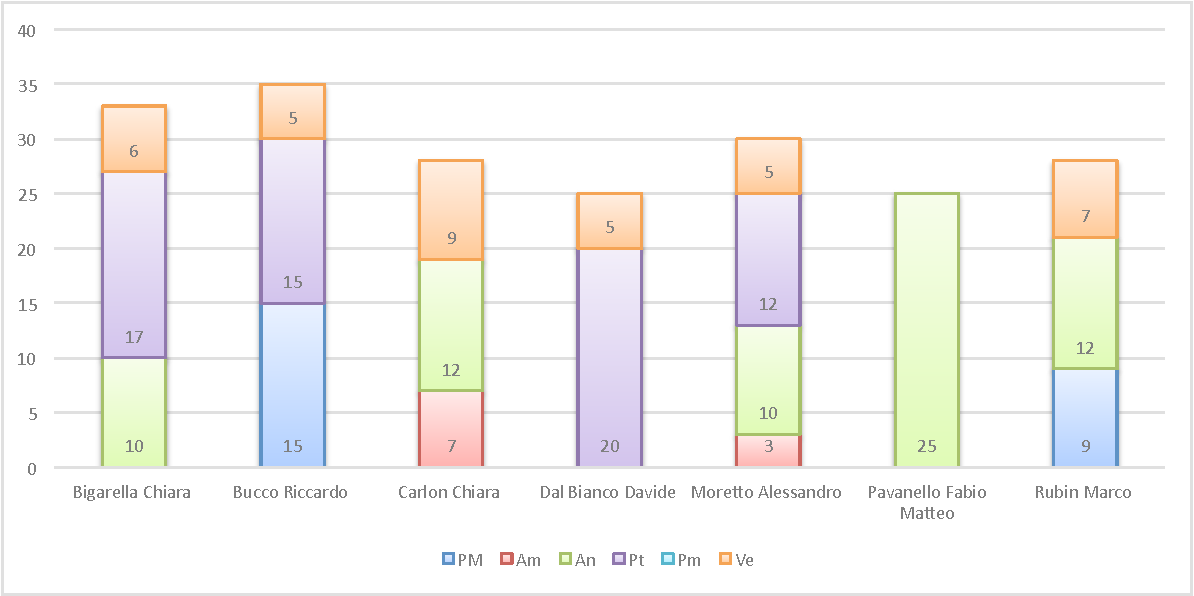
\includegraphics[width=\textwidth]{PianoDiProgetto/Pics/ChartOreFasePA.pdf}
					\caption{Bar Chart ore persona Fase PA}
				\end{figure}
			\paragraph{Prospetto economico}
				Nella \insphase{Fase PA} il costo di ogni ruolo è il seguente:
				\begin{table}[H]
					\begin{center}
						\begin{tabular}{| l | c | c |}
							\hline
							Ruolo 			& Ore 	& Costi  \\ \hline
							
							Product Manager	& 24 		& \euro{} 720,00 	\\
							Amministratore 		& 10 		& \euro{} 200,00 	\\
							Analista	 		& 69 		& \euro{} 1~725,00 	\\
							Progettista 		& 64 		& \euro{} 1~408,00  	\\
							Programmatore		& 0		& \euro{} 0,00	\\
							Verificatore		& 37 		& \euro{} 555,00 	\\ \hline \hline
							
							Totale	 		& 204 	& \euro{} 4~608,00 	\\ \hline
						\end{tabular}
					\end{center}
					\caption{Costi per ruolo Fase PA}
				\end{table}
				Riassumendo le ore per ruolo con un Cake Chart:
				\begin{figure}[H]\centering
					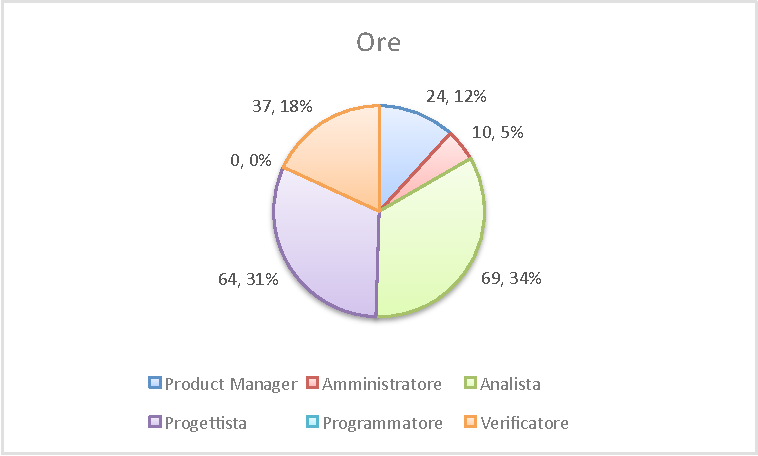
\includegraphics[width=\textwidth]{PianoDiProgetto/Pics/ChartTotOreFasePA.pdf}
					\caption{Cake Chart ore per ruolo Fase PA}
				\end{figure}
				Riassumendo i costi per ruolo con un Cake Chart:
				\begin{figure}[H]\centering
					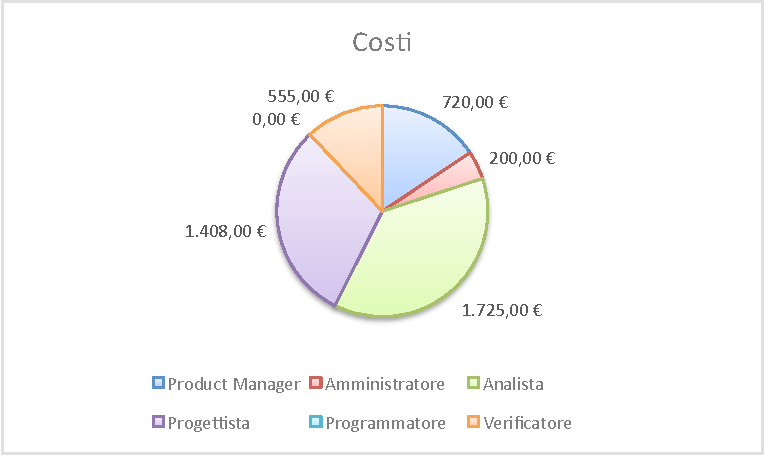
\includegraphics[width=\textwidth]{PianoDiProgetto/Pics/ChartTotCostiFasePA.pdf}
					\caption{Cake Chart costi per ruolo Fase PA}
				\end{figure}
		\subsubsection{Fase PROB}
			\paragraph{Suddivisione lavoro}
				Nella \insphase{Fase PROB} ogni componente del gruppo \groupname{} coprirà i seguenti ruoli:
				\begin{table}[H]
					\begin{center}
						\begin{tabular}{| l | c | c | c | c | c | c | c |}
							\hline
							Componente 				& PM	& Am 	& An 	& Pt 		& Pm 	& Ve 	& Ore Totali componente \\ \hline
							
							Bigarella Chiara 			& 0		& 0		& 0		& 9 		& 14 		& 8 		& 31 \\
							Bucco Riccardo 			& 0		& 0		& 0		& 7 		& 12		& 15 		& 34 \\
							Carlon Chiara	 			& 0		& 0		& 13 		& 0		& 11 		& 6 		& 30 \\
							Dal Bianco Davide 			& 17 		& 0		& 0		& 13 		& 0		& 3 		& 33 \\
							Moretto Alessandro 			& 0		& 5 		& 0		& 17 		& 4 		& 8 		& 34 \\
							Pavanello Fabio Matteo	 	& 0		& 0		& 12 		& 0		& 8 		& 13 		& 33 \\
							Rubin Marco				& 0		& 4 		& 0		& 17 		& 0		& 8 		& 29 \\ \hline \hline
							
							Ore Totali Ruolo 			& 17 		& 9 		& 25 		& 63 		& 49 		& 61 		& 224	\\ \hline
						\end{tabular}
					\end{center}
					\caption{Suddivisione ore di lavoro Fase PROB}
				\end{table}
				Riassumendo con un Bar Chart:
				\begin{figure}[H]\centering
					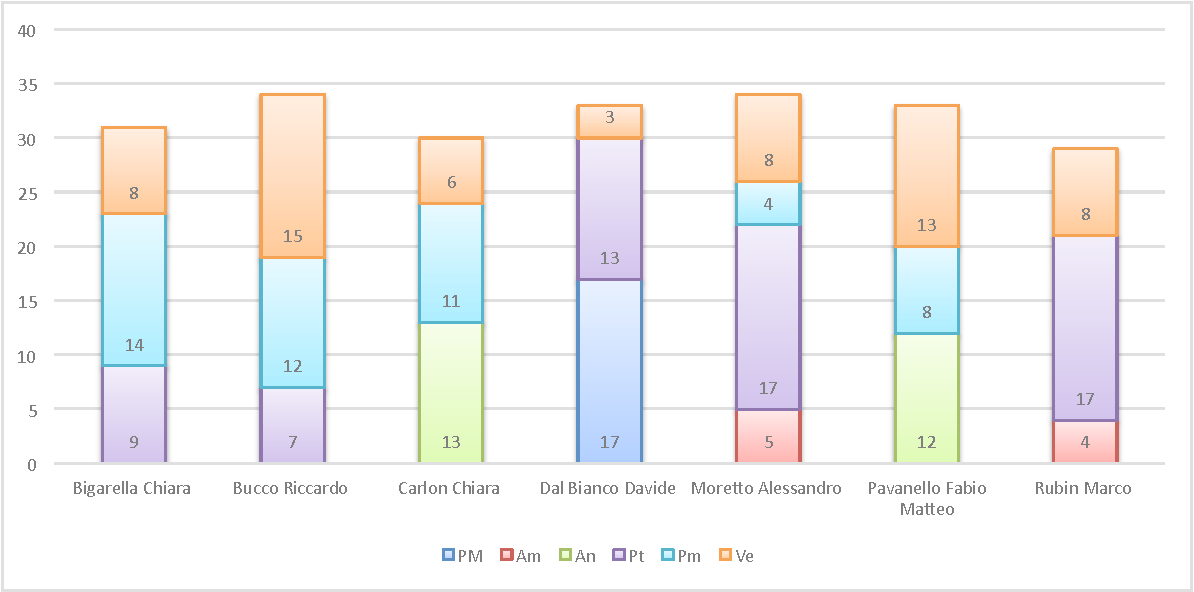
\includegraphics[width=\textwidth]{PianoDiProgetto/Pics/ChartOreFasePROB.pdf}
					\caption{Bar Chart ore persona Fase PROB}
				\end{figure}
			\paragraph{Prospetto economico}
				Nella \insphase{Fase PROB} il costo di ogni ruolo è il seguente:
				\begin{table}[H]
					\begin{center}
						\begin{tabular}{| l | c | c |}
							\hline
							Ruolo 			& Ore 	& Costi  \\ \hline
							
							Product Manager	& 17 		& \euro{} 510,00 	\\
							Amministratore 		& 9 		& \euro{} 180,00 	\\
							Analista	 		& 25 		& \euro{} 625,00 	\\
							Progettista 		& 63 		& \euro{} 1~386,00  	\\
							Programmatore		& 49 		& \euro{} 735,00 	\\
							Verificatore		& 61 		& \euro{} 915,00 	\\ \hline \hline
							
							Totale	 		& 224 	& \euro{} 4~351,00 	\\ \hline
						\end{tabular}
					\end{center}
					\caption{Costi per ruolo Fase PROB}
				\end{table}
				Riassumendo le ore per ruolo con un Cake Chart:
				\begin{figure}[H]\centering
					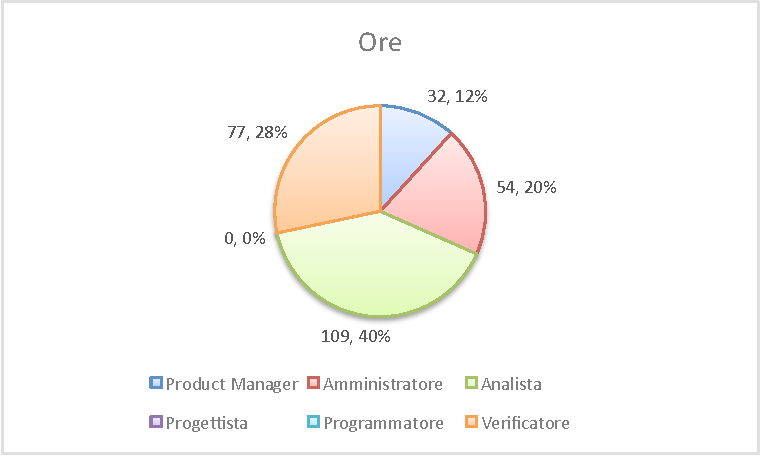
\includegraphics[width=\textwidth]{PianoDiProgetto/Pics/ChartTotOreFasePROB.pdf}
					\caption{Cake Chart ore per ruolo Fase PROB}
				\end{figure}
				Riassumendo i costi per ruolo con un Cake Chart:
				\begin{figure}[H]\centering
					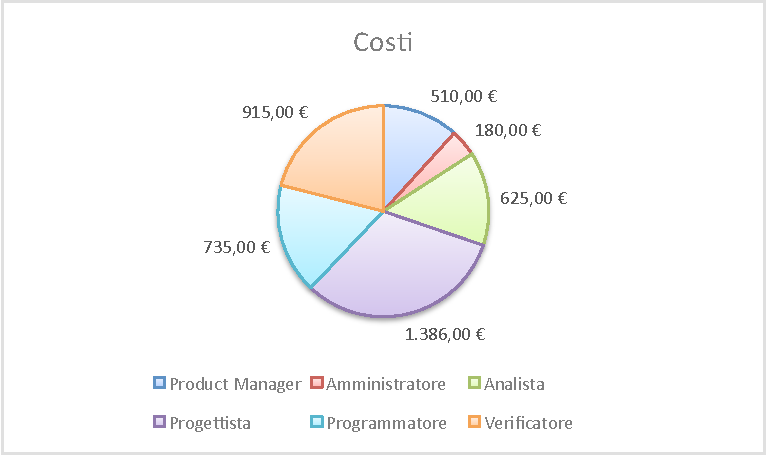
\includegraphics[width=\textwidth]{PianoDiProgetto/Pics/ChartTotCostiFasePROB.pdf}
					\caption{Cake Chart costi per ruolo Fase PROB}
				\end{figure}
		\subsubsection{Fase PRD}
			\paragraph{Suddivisione lavoro}
				Nella \insphase{Fase PRD} ogni componente del gruppo \groupname{} coprirà i seguenti ruoli:
				\begin{table}[H]
					\begin{center}
						\begin{tabular}{| l | c | c | c | c | c | c | c |}
							\hline
							Componente 				& PM	& Am	& An 	& Pt 		& Pm 	& Ve 	& Ore Totali componente \\ \hline
							
							Bigarella Chiara 			& 10 		& 0		& 0		& 0		& 3 		& 0		& 13 \\
							Bucco Riccardo 			& 0		& 0		& 0		& 0		& 2		& 12 		& 14 \\
							Carlon Chiara	 			& 0		& 2 		& 0		& 4 		& 2 		& 8 		& 16 \\
							Dal Bianco Davide 			& 0		& 0		& 0		& 0		& 5 		& 8 		& 13 \\
							Moretto Alessandro 			& 0		& 0		& 13 		& 0		& 0		& 0		& 13 \\
							Pavanello Fabio Matteo	 	& 0		& 0		& 0		& 0		& 3 		&11 		& 14 \\
							Rubin Marco				& 0		& 3 		& 0		& 6 		& 3 		& 6		& 18 \\ \hline \hline
							
							Ore Totali Ruolo 			& 10 		& 5 		& 13 		& 10 		& 18 		& 45 		& 101\\ \hline
						\end{tabular}
					\end{center}
					\caption{Suddivisione ore di lavoro Fase PRD}
				\end{table}
				Riassumendo con un Bar Chart:
				\begin{figure}[H]\centering
					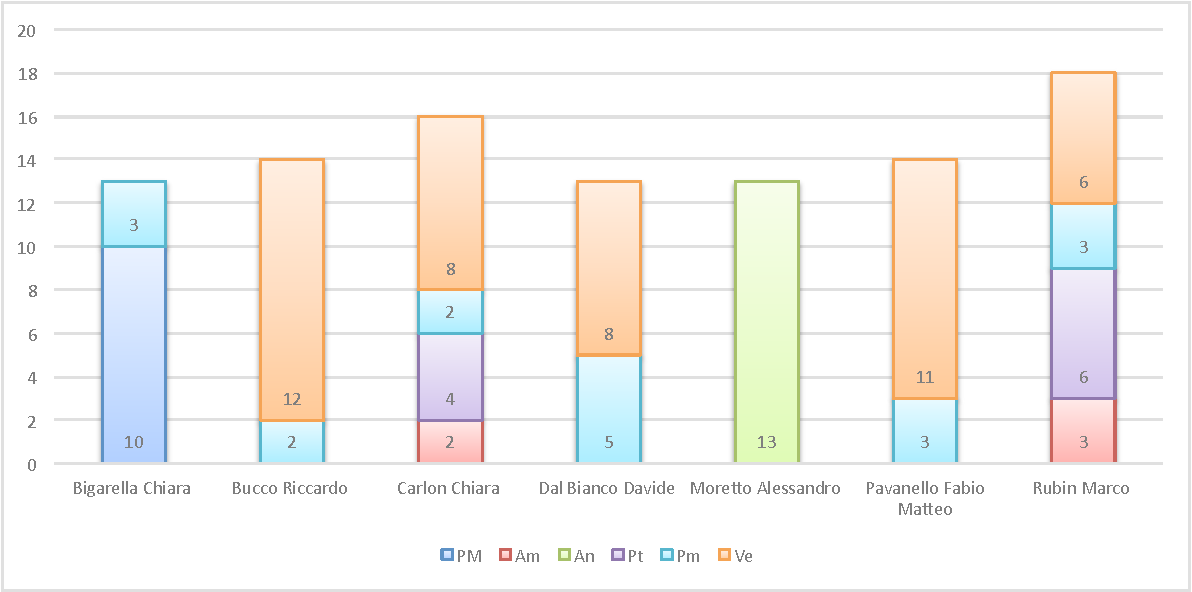
\includegraphics[width=\textwidth]{PianoDiProgetto/Pics/ChartOreFasePRD.pdf}
					\caption{Bar Chart ore persona Fase PRD}
				\end{figure}
			\paragraph{Prospetto economico}
				Nella \insphase{Fase PRD} il costo di ogni ruolo è il seguente:
				\begin{table}[H]
					\begin{center}
						\begin{tabular}{| l | c | c |}
							\hline
							Ruolo 			& Ore 	& Costi  \\ \hline
							
							Product Manager	& 10 		& \euro{} 300,00 	\\
							Amministratore 		& 5 		& \euro{} 100,00 	\\
							Analista	 		& 13 		& \euro{} 325,00 	\\
							Progettista 		& 10 		& \euro{} 220,00  	\\
							Programmatore		& 18		& \euro{} 270,00 	\\
							Verificatore		& 45 		& \euro{} 675,00 	\\ \hline \hline
							
							Totale	 		& 101 	& \euro{} 1~890,00 	\\ \hline
						\end{tabular}
					\end{center}
					\caption{Costi per ruolo Fase PRD}
				\end{table}
				Riassumendo le ore per ruolo con un Cake Chart:
				\begin{figure}[H]\centering
					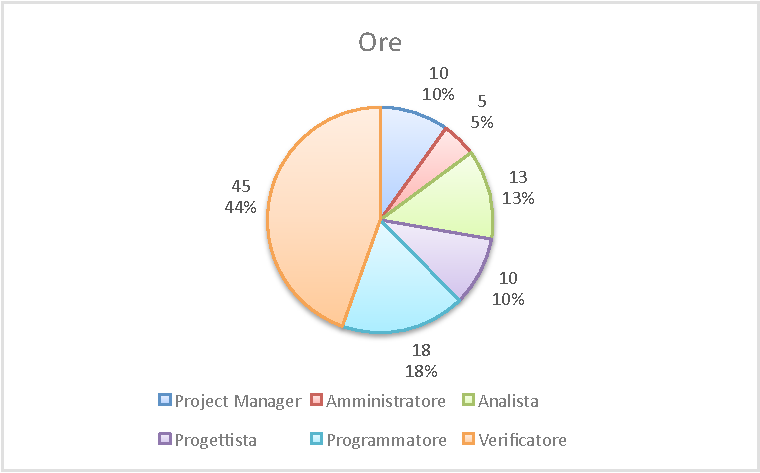
\includegraphics[width=\textwidth]{PianoDiProgetto/Pics/ChartTotOreFasePRD.pdf}
					\caption{Cake Chart ore per ruolo Fase PRD}
				\end{figure}
				Riassumendo i costi per ruolo con un Cake Chart:
				\begin{figure}[H]\centering
					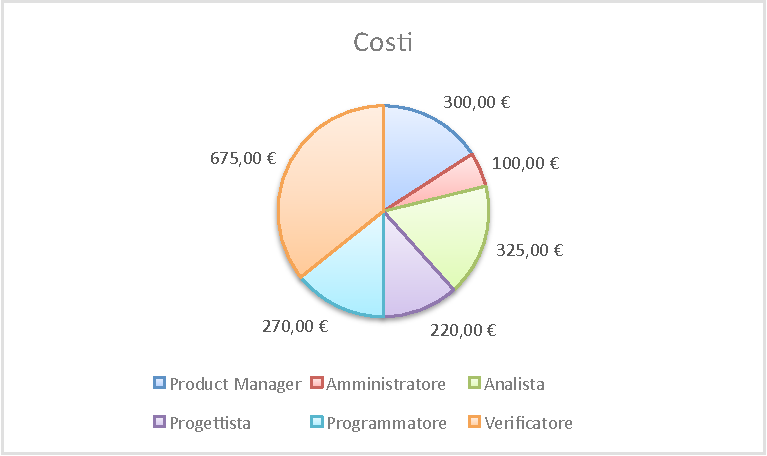
\includegraphics[width=\textwidth]{PianoDiProgetto/Pics/ChartTotCostiFasePRD.pdf}
					\caption{Cake Chart costi per ruolo Fase PRD}
				\end{figure}
		\subsubsection{Fase PROP}
			\paragraph{Suddivisione lavoro}
				Nella \insphase{Fase PROP} ogni componente del gruppo \groupname{} coprirà i seguenti ruoli:
				\begin{table}[H]
					\begin{center}
						\begin{tabular}{| l | c | c | c | c | c | c | c |}
							\hline
							Componente 				& PM	& Am 	& An 	& Pt 		& Pm 	& Ve 	& Ore Totali componente \\ \hline
							
							Bigarella Chiara 			& 0		& 0		& 0		& 6 		& 0		& 8 		& 14 \\
							Bucco Riccardo 			& 0		& 0		& 0		& 4 		& 0		& 7 		& 11 \\
							Carlon Chiara	 			& 0		& 5 		& 0		& 10 		& 0		& 3 		& 18 \\
							Dal Bianco Davide 			& 0		& 0		& 0		& 0		& 12 		& 9 		& 21 \\
							Moretto Alessandro 			& 0		& 0		& 0		& 0		& 11 		& 5		& 16 \\
							Pavanello Fabio Matteo	 	& 13 		& 0		& 0		& 0		& 5 		& 4 		& 22 \\
							Rubin Marco				& 0		& 0		& 13 		& 0		& 0		& 4 		& 17 \\ \hline \hline
							
							Ore Totali Ruolo 			& 13 		& 5 		& 13 		& 20 		& 28 		& 40 		& 119\\ \hline
						\end{tabular}
					\end{center}
					\caption{Suddivisione ore di lavoro Fase PROP}
				\end{table}
				Riassumendo con un Bar Chart:
				\begin{figure}[H]\centering
					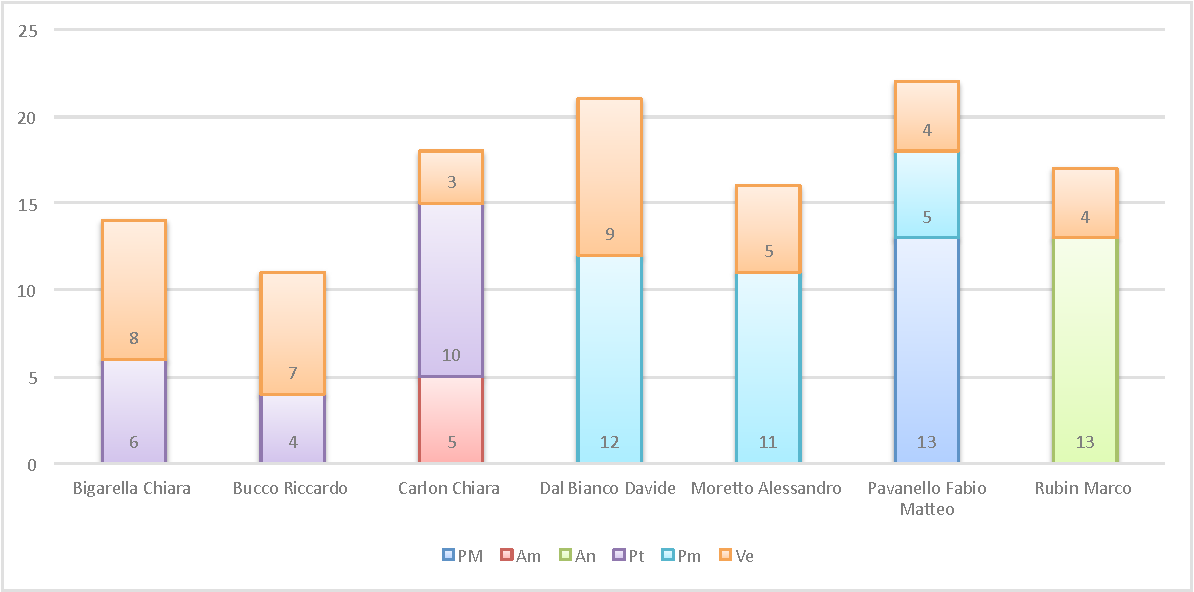
\includegraphics[width=\textwidth]{PianoDiProgetto/Pics/ChartOreFasePROP.pdf}
					\caption{Bar Chart ore persona Fase PROP}
				\end{figure}
			\paragraph{Prospetto economico}
				Nella \insphase{Fase PROP} il costo di ogni ruolo è il seguente:
				\begin{table}[H]
					\begin{center}
						\begin{tabular}{| l | c | c |}
							\hline
							Ruolo 			& Ore 		& Costi  \\ \hline
							
							Product Manager	& 13 		& \euro{} 390,00 	\\
							Amministratore 		& 5 		& \euro{} 100,00 	\\
							Analista	 		& 13 		& \euro{} 325,00 	\\
							Progettista 		& 20 		& \euro{} 440,00  	\\
							Programmatore		& 28 		& \euro{} 420,00 	\\
							Verificatore		& 40 		& \euro{} 600,00 	\\ \hline \hline
							
							Totale	 		& 119 	& \euro{} 2~275,00 	\\ \hline
						\end{tabular}
					\end{center}
					\caption{Costi per ruolo Fase PROP}
				\end{table}
				Riassumendo le ore per ruolo con un Cake Chart:
				\begin{figure}[H]\centering
					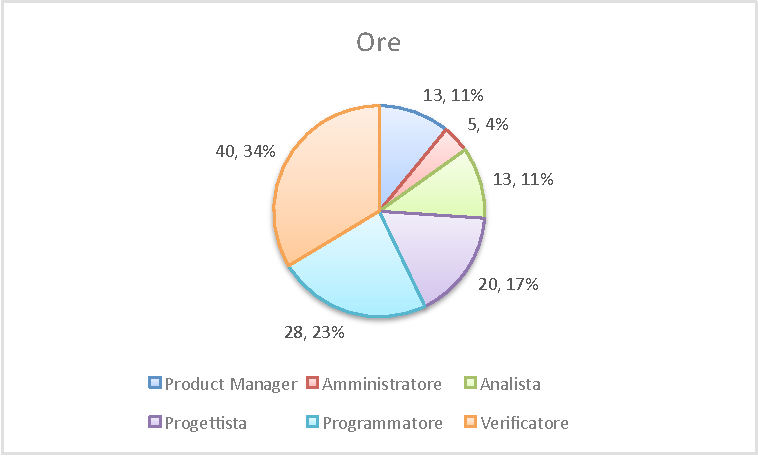
\includegraphics[width=\textwidth]{PianoDiProgetto/Pics/ChartTotOreFasePROP.pdf}
					\caption{Cake Chart ore per ruolo Fase PROP}
				\end{figure}
				Riassumendo i costi per ruolo con un Cake Chart:
				\begin{figure}[H]\centering
					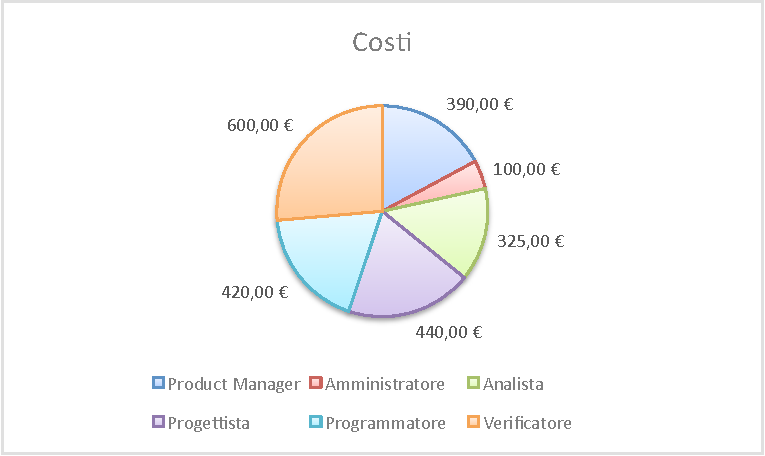
\includegraphics[width=\textwidth]{PianoDiProgetto/Pics/ChartTotCostiFasePROP.pdf}
					\caption{Cake Chart costi per ruolo Fase PROP}
				\end{figure}
		\subsubsection{Fase V}
			\paragraph{Suddivisione lavoro}
				Nella \insphase{Fase V} ogni componente del gruppo \groupname{} coprirà i seguenti ruoli:
				\begin{table}[H]
					\begin{center}
						\begin{tabular}{| l | c | c | c | c | c | c | c |}
							\hline
							Componente 				& PM	& Am 	& An 	& Pt 		& Pm 	& Ve 	& Ore Totali componente \\ \hline
							
							Bigarella Chiara 			& 0		& 0		& 0		& 0		& 5 		& 9 		& 14 \\
							Bucco Riccardo 			& 0		& 0		& 0		& 0		& 7		& 4 		& 11 \\
							Carlon Chiara	 			& 10 		& 0		& 0		& 0		& 0		& 3 		& 13 \\
							Dal Bianco Davide 			& 0		& 0		& 0		& 0		& 0		& 13 		& 13 \\
							Moretto Alessandro 			& 0		& 3 		& 0		& 0		& 0		& 9 		& 12 \\
							Pavanello Fabio Matteo	 	& 0		& 0		& 0		& 9 		& 0		& 2 		& 11 \\
							Rubin Marco				& 0		& 0		& 0		& 0		& 5 		& 8 		& 13 \\ \hline \hline
							
							Ore Totali Ruolo 			& 10 		& 3 		& 0		& 9 		& 17 		& 48 		& 87\\ \hline
						\end{tabular}
					\end{center}
					\caption{Suddivisione ore di lavoro Fase V}
				\end{table}
				Riassumendo con un Bar Chart:
				\begin{figure}[H]\centering
					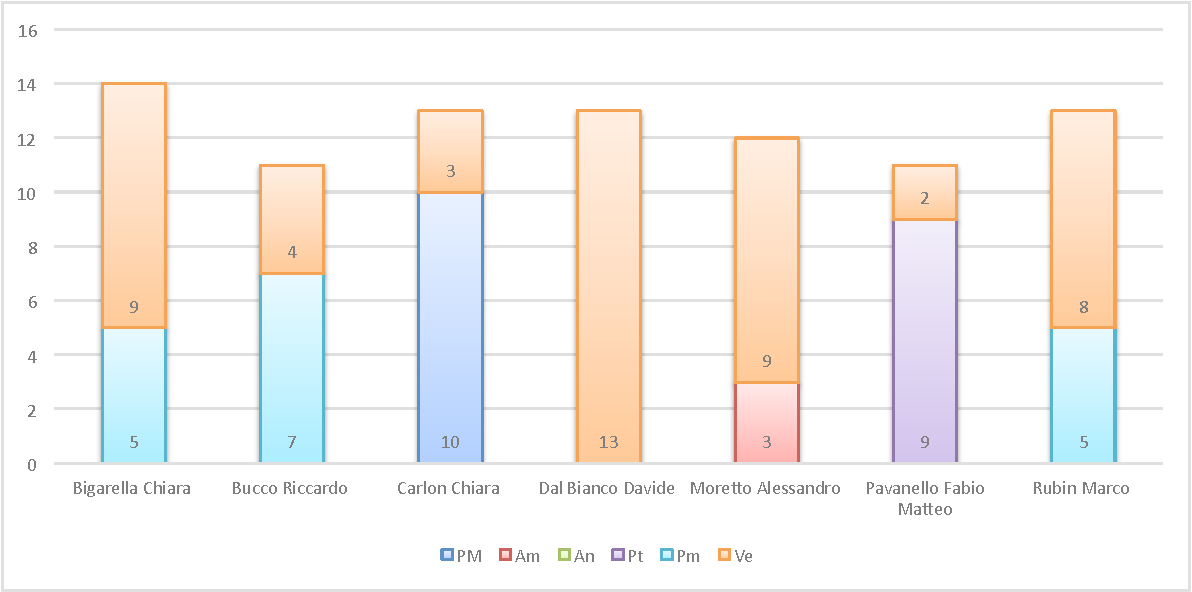
\includegraphics[width=\textwidth]{PianoDiProgetto/Pics/ChartOreFaseV.pdf}
					\caption{Bar Chart ore persona Fase V}
				\end{figure}
			\paragraph{Prospetto economico}
				Nella \insphase{Fase V} il costo di ogni ruolo è il seguente:
				\begin{table}[H]
					\begin{center}
						\begin{tabular}{| l | c | c |}
							\hline
							Ruolo 			& Ore 	& Costi  \\ \hline
							
							Product Manager	& 10 		& \euro{} 300,00 	\\
							Amministratore 		& 3 		& \euro{} 60,00 	\\
							Analista	 		& 0		& \euro{} 0,00	\\
							Progettista 		& 9 		& \euro{} 198,00  	\\
							Programmatore		& 17 		& \euro{} 225,00 	\\
							Verificatore		& 48 		& \euro{} 720,00 	\\ \hline \hline
							
							Totale	 		& 87 		& \euro{} 1~533,00 	\\ \hline
						\end{tabular}
					\end{center}
					\caption{Costi per ruolo Fase V}
				\end{table}
				Riassumendo le ore per ruolo con un Cake Chart:
				\begin{figure}[H]\centering
					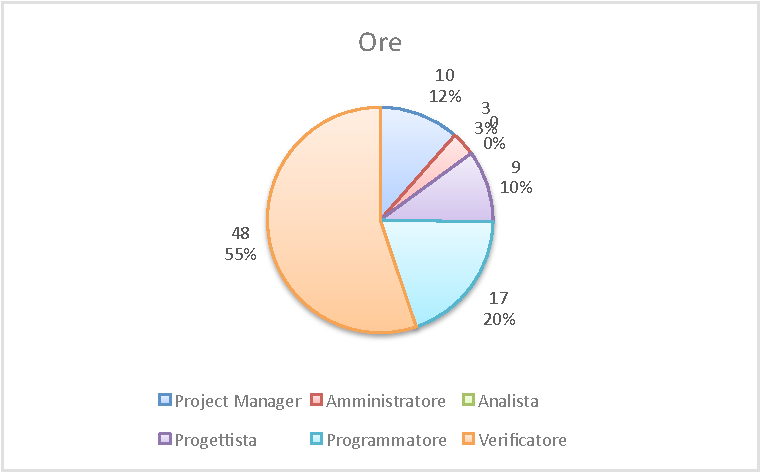
\includegraphics[width=\textwidth]{PianoDiProgetto/Pics/ChartTotOreFaseV.pdf}
					\caption{Cake Chart ore per ruolo Fase V}
				\end{figure}
				Riassumendo i costi per ruolo con un Cake Chart:
				\begin{figure}[H]\centering
					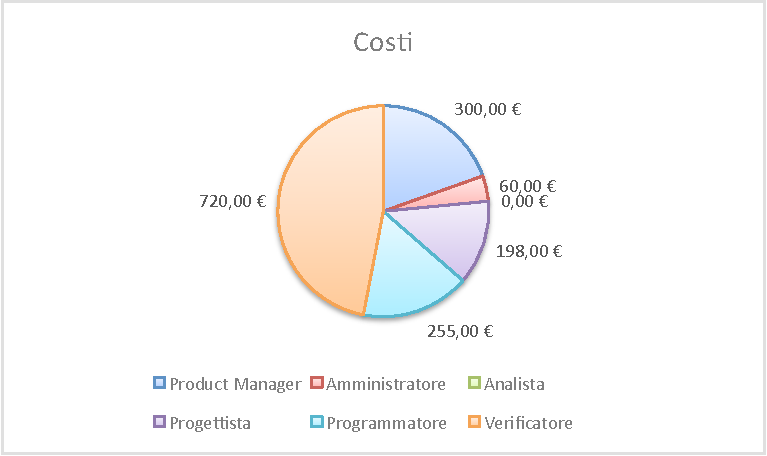
\includegraphics[width=\textwidth]{PianoDiProgetto/Pics/ChartTotCostiFaseV.pdf}
					\caption{Cake Chart costi per ruolo Fase V}
				\end{figure}
	\subsection{Resoconto}
	\subsubsection{Ore totali}			
		\paragraph{Suddivisione lavoro}
				La suddivisione delle ore di impegno per ruolo di ogni componente del gruppo \groupname{} saranno le seguenti:
				\begin{table}[H]
					\begin{center}
						\begin{tabular}{| l | c | c | c | c | c | c | c |}
							\hline
							Componente 				& PM	& Am 	& An 	& Pt 		& Pm 	& Ve 	& Ore Totali componente \\ \hline
							
							Bigarella Chiara 			& 10		& 12 		& 40 		& 32		& 22		& 44 		& 160 \\
							Bucco Riccardo 			& 15		& 11 		& 30 		& 26		& 21		& 58 		& 161 \\
							Carlon Chiara	 			& 17 		& 20 		& 37 		& 14		& 13		& 48 		& 149 \\
							Dal Bianco Davide 			& 17		& 20 		& 25 		& 33		& 17		& 48 		& 160 \\
							Moretto Alessandro 			& 25 		& 11		& 35 		& 29		& 15		& 43 		& 158 \\
							Pavanello Fabio Matteo	 	& 13		& 5 		& 46 		& 9		& 16		& 63 		& 152 \\
							Rubin Marco				& 16 		& 26 		& 28 		& 23		& 8		& 51 		& 152 \\ \hline \hline
							
							Ore Totali Ruolo 			& 113 	& 105	& 241 	& 166	& 112		& 355 	& 1~092 \\ \hline
						\end{tabular}
					\end{center}
					\caption{Suddivisione ore totali}
				\end{table}
				Riassumendo con un Bar Chart:
				\begin{figure}[H]\centering
					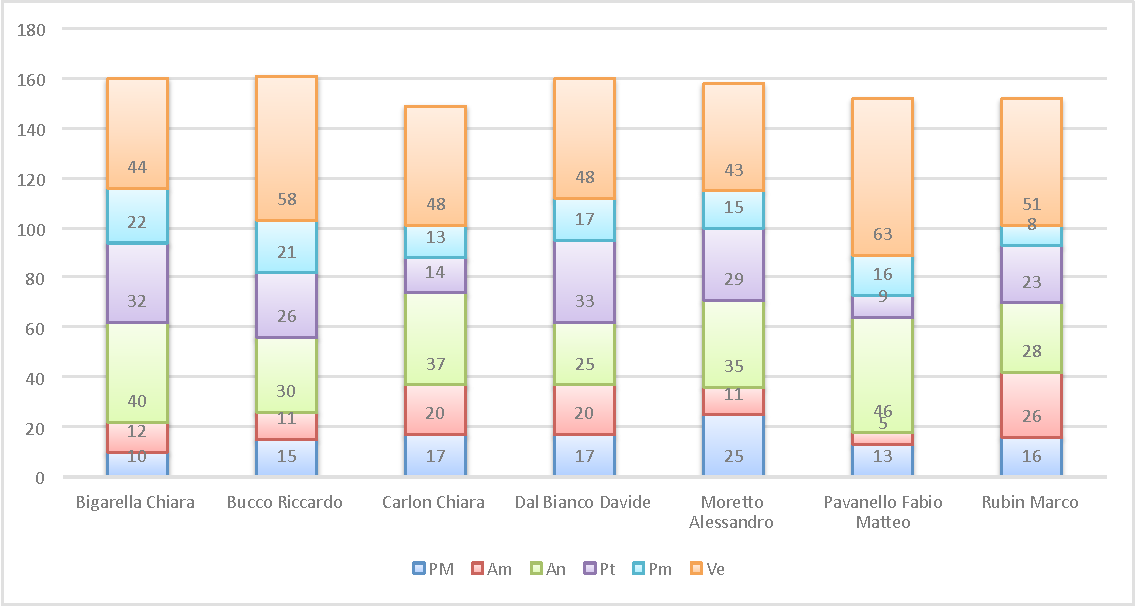
\includegraphics[width=\textwidth]{PianoDiProgetto/Pics/ChartOreTot.pdf}
					\caption{Bar Chart ore totali}
				\end{figure}
			\paragraph{Prospetto economico}
				I costi totali (rendicontati o no) per ogni ruolo comprende sia le ore di formazione a carico del \groupname{}, sia le ore rendicontate, che verranno addebitate al proponente.\\
				L'investimento per ogni ruolo è il seguente:
				\begin{table}[H]
					\begin{center}
						\begin{tabular}{| l | c | c |}
							\hline
							Ruolo 			& Ore 	& Costi  \\ \hline
							
							Product Manager	& 113 	& \euro{} 3~390,00 	\\
							Amministratore 		& 105 	& \euro{} 2~100,00 	\\
							Analista	 		& 241 	& \euro{} 6~025,00 	\\
							Progettista 		& 166	& \euro{} 3~652,00 	\\
							Programmatore		& 112	& \euro{} 1~680,00	\\
							Verificatore		& 355 	& \euro{} 5~325,00 	\\ \hline \hline
							
							Totale	 		& 1092 	& \euro{} 22~172,00 	\\ \hline
						\end{tabular}
					\end{center}
					\caption{Costi totali per ruolo}
				\end{table}
				Riassumendo le ore totali per ruolo con un Cake Chart:
				\begin{figure}[H]\centering
					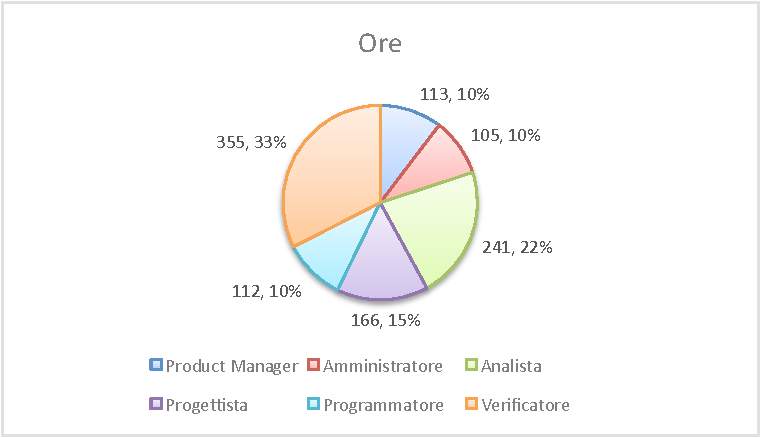
\includegraphics[width=\textwidth]{PianoDiProgetto/Pics/ChartTotOre.pdf}
					\caption{Cake Chart ore totali}
				\end{figure}
				Riassumendo i costi per ruolo con un Cake Chart:
				\begin{figure}[H]\centering
					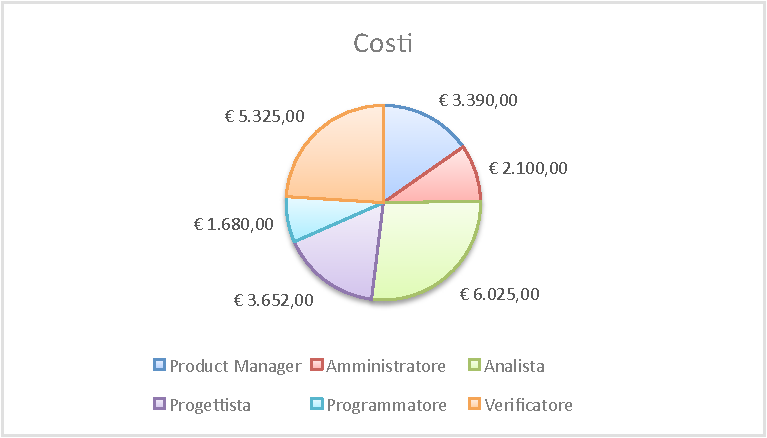
\includegraphics[width=\textwidth]{PianoDiProgetto/Pics/ChartTotCosti.pdf}
					\caption{Cake Chart costi totali per ruolo}
				\end{figure}
		\subsubsection{Ore totali di investimento}
		Le ore di investimento sono le ore svolte non rendicontate. Durante la \insphase{Fase A} e la \insphase{Fase AD} le ore effettuate non sono a carico del proponente.
			\paragraph{Suddivisione lavoro}
				La suddivisione delle ore di investimento per ruolo di ogni componente del gruppo \groupname{} saranno le seguenti:
				\begin{table}[H]
					\begin{center}
						\begin{tabular}{| l | c | c | c | c | c | c | c |}
							\hline
							Componente 				& PM	& Am 	& An 	& Pt 		& Pm 	& Ve 	& Ore Totali componente \\ \hline
							
							Bigarella Chiara 			& 0		& 12 		& 30 		& 0		& 0		& 13 		& 55 \\
							Bucco Riccardo 			& 0		& 11 		& 30 		& 0		& 0		& 15 		& 56 \\
							Carlon Chiara	 			& 7 		& 6 		& 12 		& 0		& 0		& 19 		& 44 \\
							Dal Bianco Davide 			& 0		& 20 		& 25 		& 0		& 0		& 10 		& 55 \\
							Moretto Alessandro 			& 25 		& 0		& 12 		& 0		& 0		& 16 		& 53 \\
							Pavanello Fabio Matteo	 	& 0		& 5 		& 9 		& 0		& 0		& 33 		& 47 \\
							Rubin Marco				& 7 		& 19 		& 3 		& 0		& 0		& 18 		& 47 \\ \hline \hline
							
							Ore Totali Ruolo 			& 39 		& 73 		& 121 	& 0		& 0		& 124 	& 357\\ \hline
						\end{tabular}
					\end{center}
					\caption{Suddivisione ore totali di investimento}
				\end{table}
				Riassumendo con un Bar Chart:
				\begin{figure}[H]\centering
					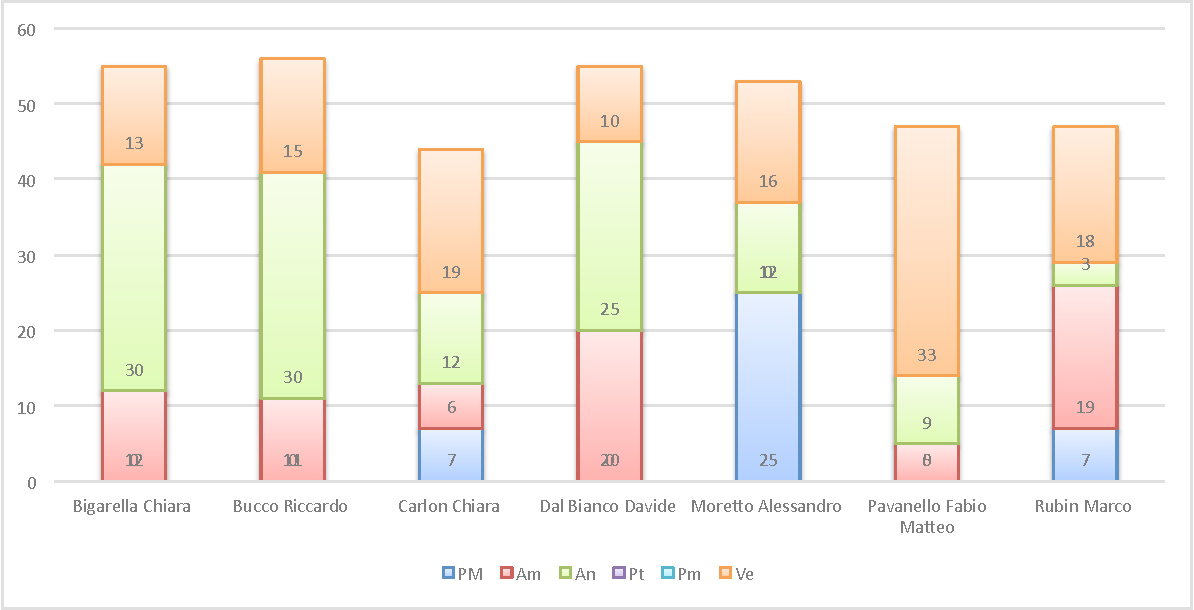
\includegraphics[width=\textwidth]{PianoDiProgetto/Pics/ChartOreInvest.pdf}
					\caption{Bar Chart ore totali di investimento}
				\end{figure}
			\paragraph{Prospetto economico}
				L'investimento per ogni ruolo è il seguente:
				\begin{table}[H]
					\begin{center}
						\begin{tabular}{| l | c | c |}
							\hline
							Ruolo 			& Ore 		& Costi  \\ \hline
							
							Product Manager	& 39 		& \euro{} 1~170,00 	\\
							Amministratore 		& 73 		& \euro{} 1~460,00 	\\
							Analista	 		& 121 	& \euro{} 3~025,00 	\\
							Progettista 		& 0		& \euro{} 0,00 	\\
							Programmatore		& 0		& \euro{} 0,00	\\
							Verificatore		& 124 	& \euro{} 1~860,00 	\\ \hline \hline
							
							Totale	 		& 357 	& \euro{} 7~515,00 	\\ \hline
						\end{tabular}
					\end{center}
					\caption{Investimento per ruolo}
				\end{table}
				Riassumendo le ore di investimento per ruolo con un Cake Chart:
				\begin{figure}[H]\centering
					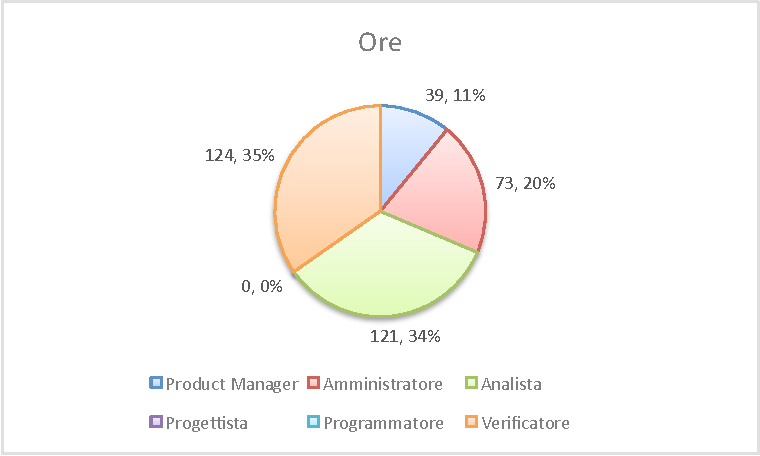
\includegraphics[width=\textwidth]{PianoDiProgetto/Pics/ChartTotOreInvest.pdf}
					\caption{Cake Chart ore di investimento}
				\end{figure}
				Riassumendo i costi per ruolo con un Cake Chart:
				\begin{figure}[H]\centering
					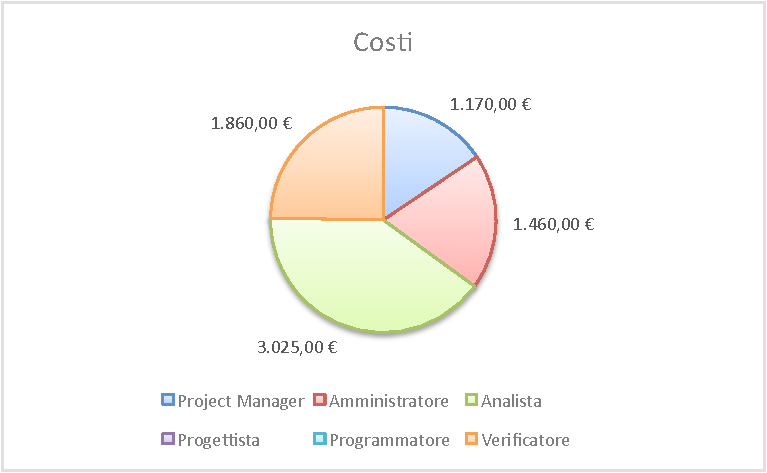
\includegraphics[width=\textwidth]{PianoDiProgetto/Pics/ChartTotCostiInvest.pdf}
					\caption{Cake Chart investimento per ruolo}
				\end{figure}
		\subsubsection{Ore rendicontate}
			Le ore rendicontate sono le ore svolte a carico del proponente.
			\paragraph{Suddivisione lavoro}
				La suddivisione delle ore rendicontate per ruolo di ogni componente del gruppo \groupname{} saranno le seguenti:
				\begin{table}[H]
					\begin{center}
						\begin{tabular}{| l | c | c | c | c | c | c | c |}
							\hline
							Componente 				& PM	& Am 	& An 	& Pt 		& Pm 	& Ve 	& Ore Totali componente \\ \hline
							
							Bigarella Chiara 			& 10 		& 0		& 10 		& 32 		& 22 		& 31 		& 105 \\
							Bucco Riccardo 			& 15 		& 0		& 0		& 26 		& 21		& 43 		& 105 \\
							Carlon Chiara	 			& 10 		& 14 		& 25 		& 14 		& 13 		& 29 		& 105 \\
							Dal Bianco Davide 			& 17 		& 0		& 0		& 33 		& 17 		& 38 		& 105 \\
							Moretto Alessandro 			& 0		& 11 		& 23 		& 29 		& 15 		& 27 		& 105 \\
							Pavanello Fabio Matteo	 	& 13 		& 0		& 37 		& 9 		& 16 		& 30 		& 105 \\
							Rubin Marco				& 9 		& 7 		& 25 		& 23 		& 8 		& 33		& 105 \\ \hline \hline
							
							Ore Totali Ruolo 			& 74 		& 32 		& 120 	& 166 	& 112 	& 231 	& 735\\ \hline
						\end{tabular}
					\end{center}
					\caption{Suddivisione ore totali rendicontate}
				\end{table}
				Riassumendo con un Bar Chart:
				\begin{figure}[H]\centering
					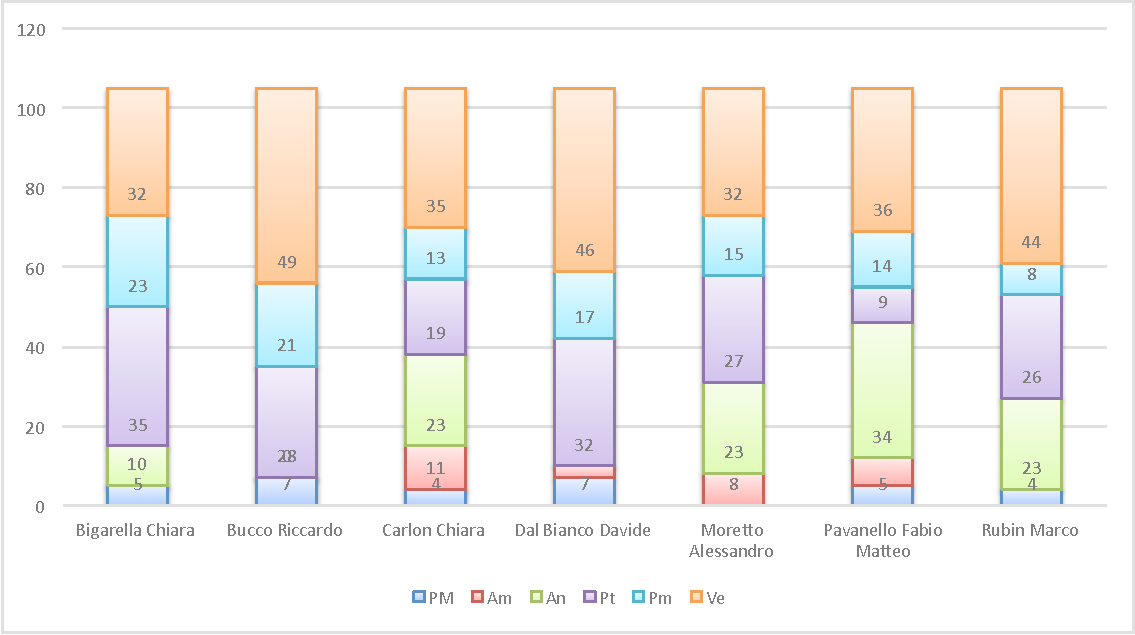
\includegraphics[width=\textwidth]{PianoDiProgetto/Pics/ChartOreRendic.pdf}
					\caption{Bar Chart ore totali rendicontate}
				\end{figure}
			\paragraph{Prospetto economico}
				Le ore rendicontate per ogni ruolo sono le seguenti:
				\begin{table}[H]
					\begin{center}
						\begin{tabular}{| l | c | c |}
							\hline
							Ruolo 			& Ore 		& Costi  \\ \hline
							
							Product Manager	& 74 			& \euro{} 2~220,00 	\\
							Amministratore 		& 32 			& \euro{} 640,00 	\\
							Analista	 		& 120 		& \euro{} 3~000,00 	\\
							Progettista 		& 166 		& \euro{} 3~652,00  	\\
							Programmatore		& 112 		& \euro{} 1~680,00 	\\
							Verificatore		& 231 		& \euro{} 3~465,00 	\\ \hline \hline
							
							Totale	 		& 735 		& \euro{} 14~657,00 	\\ \hline
						\end{tabular}
					\end{center}
					\caption{Spese rendicontate per ruolo}
				\end{table}
				Riassumendo le ore rendicontate per ruolo con un Cake Chart:
				\begin{figure}[H]\centering
					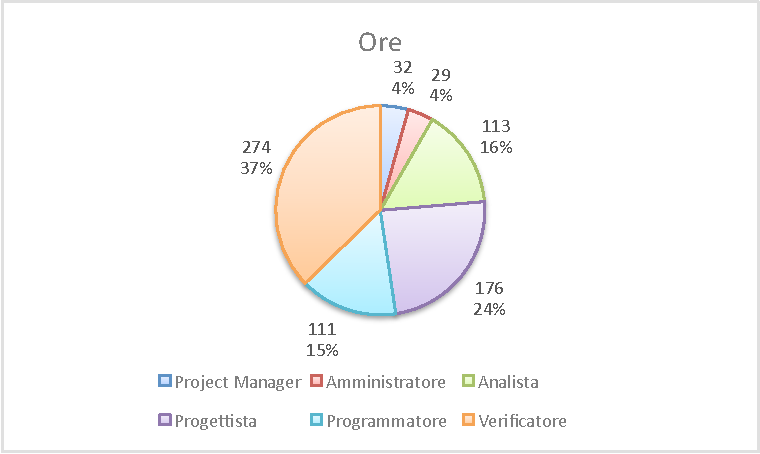
\includegraphics[width=\textwidth]{PianoDiProgetto/Pics/ChartTotOreRendic.pdf}
					\caption{Cake Chart ore rendicontate}
				\end{figure}
				Riassumendo i costi rendicontati per ruolo con un Cake Chart:
				\begin{figure}[H]\centering
					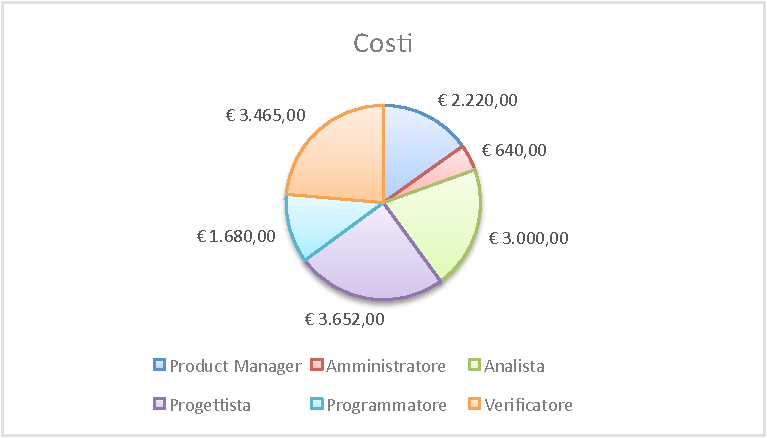
\includegraphics[width=\textwidth]{PianoDiProgetto/Pics/ChartTotCostiRendic.pdf}
					\caption{Cake Chart spese rendicontate per ruolo}
				\end{figure}
		\subsubsection{Conclusione}
			Il costo totale del progetto è di \euro{} 14~657,00.
